%PAGINA 1

\begin{frame}
    \frametitle{Trayectoria de un HAB}
    Para analizar la trayectoria, empleamos el software de la Universidad de Cambridge, CUSF, que proporciona datos detallados de latitud, longitud y altitud con marcas de tiempo minuto a minuto (ver Fig. \ref{fig:ruta}).    
    \begin{figure}[H]
        \centering
        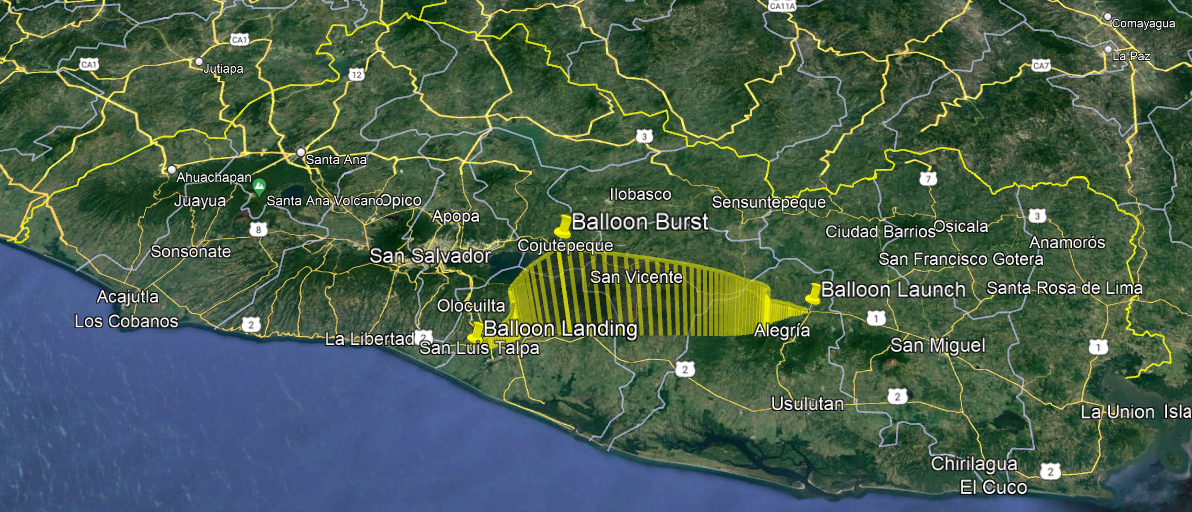
\includegraphics[width=0.75\textwidth]{ruta.png} % Ajusta el tamaño según sea necesario
        \mycaption{Simulación de Trayectoria}
        \label{fig:ruta}
    \end{figure}
    
\end{frame}

%PAGINA 2

\begin{frame}
    \frametitle{Condiciones Ambientales}

Integrando el estándar ISA con datos del CUSF mejora el análisis de variables como temperatura y presión, permitiendo predecir valores límite y tasas de cambio (ver Fig. \ref{fig:enviromentalV}).
      \begin{figure}[H]
        \centering
        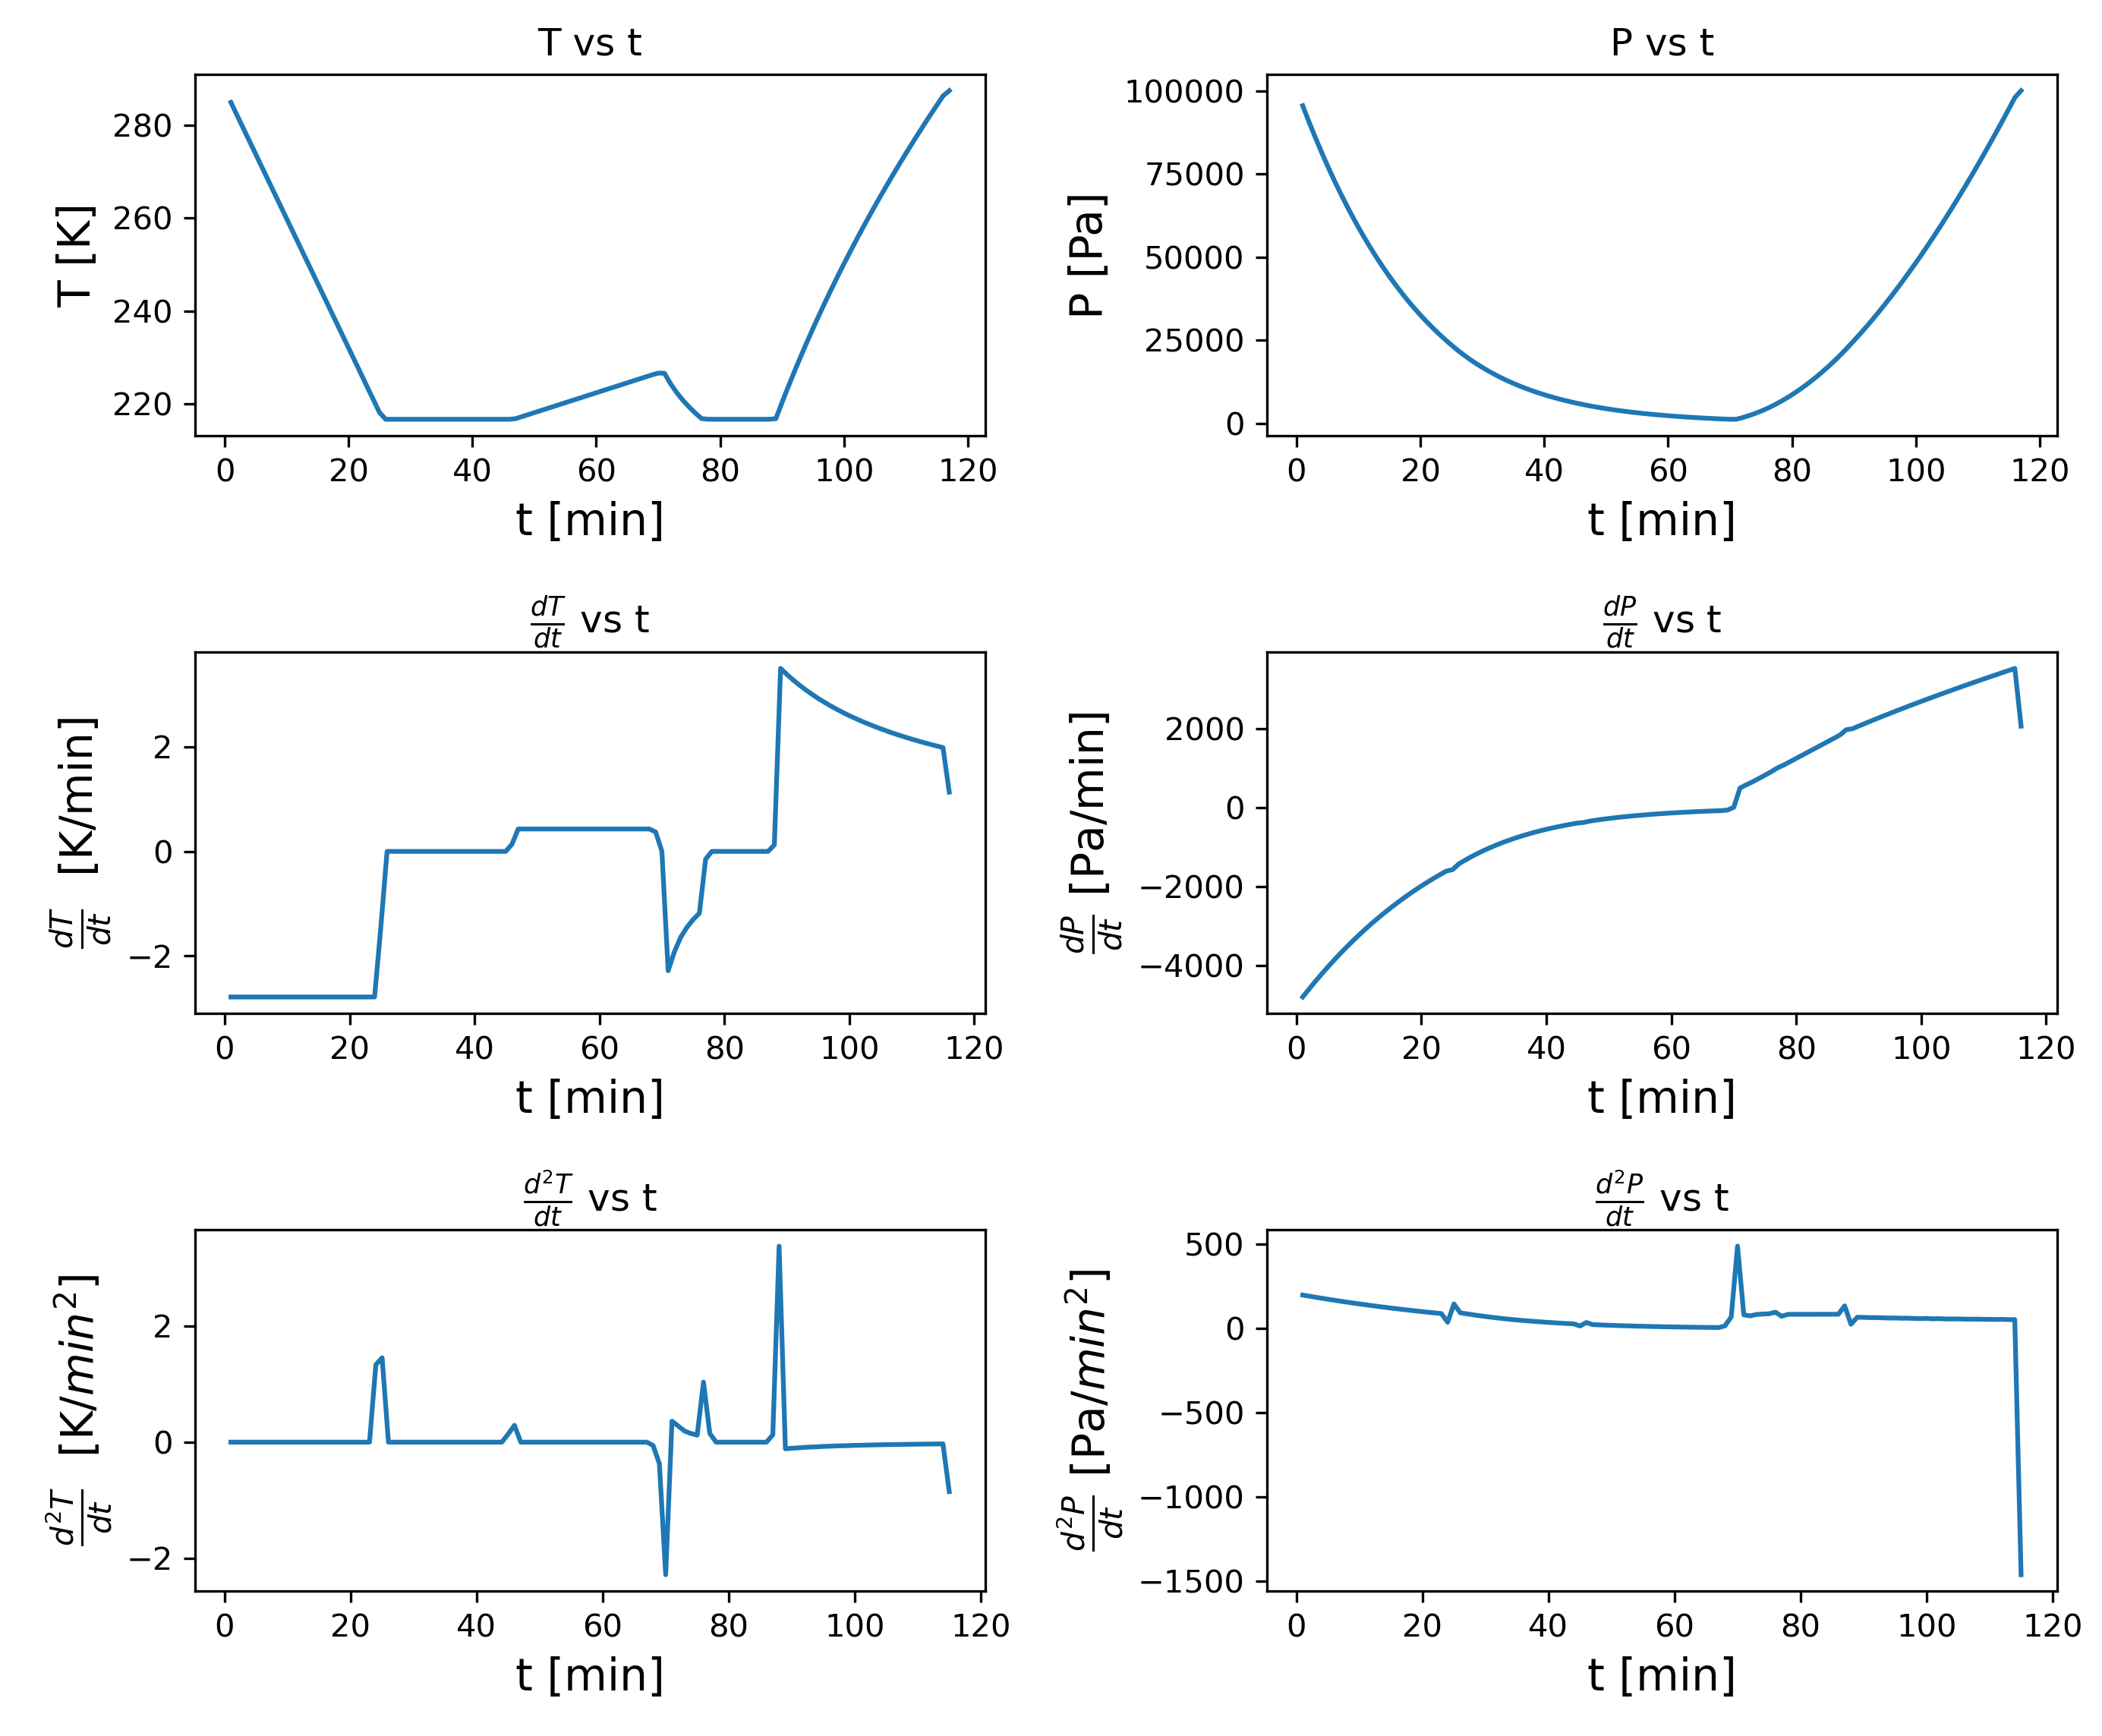
\includegraphics[width=0.75\textwidth]{EnviromentalVariables.png} % Ajusta el tamaño según sea necesario
        \mycaption{Variables atmosféricas en trayectoria de HAB}
        \label{fig:enviromentalV}
    \end{figure}
    
\end{frame}

% PAGINA 3


\begin{frame}
\frametitle{Condiciones Ambientales}

Las condiciones extremas en la estratósfera pueden alcanzar -56.50\textdegree{}C y 1.20\% de la presión atmosférica estándar. Se observaron razones de cambio máximas de -2.78\textdegree{}C por minuto y una pérdida de presión atmosférica del 4.74\% por minuto.\\ 
\vspace*{0.5 cm}
Estudios como el experimento TASEC-Lab \cite{TASEC} no solo validan estos datos, sino que también identifican una franja crítica alrededor de los 11 km de altitud, cerca de la tropopausa, con notables variaciones térmicas, un aspecto crucial para la selección de componentes y sistemas de control térmico.

   
\end{frame}



% PAGINA 4

\begin{frame}
\frametitle{Presupuesto Energético}

\begin{table}[!ht]
    \centering
    \caption{Cuadro de cargas para bus 3.3v}
    \label{tab:cuadro-cargas1}
    \resizebox{\columnwidth}{!}{% Escala la tabla para que se ajuste al ancho de la columna
    \begin{tabular}{llllllll}
    \hline
    \textbf{Descripción} & \textbf{Cantidad} & \textbf{Subsistema} & \textbf{I [mA]} & \textbf{P [W]} & \textbf{t [h]} & \textbf{E [Wh]} & \textbf{Q [mAh]} \\
    \hline
    MCU 1 & 1 unidad & Telemetría & 93.00 & 0.31 & 6.00 & 1.84 & 558 \\ 
    LoRa & 1 unidad & Telemetría & 630.00 & 2.08 & 6.00 & 12.47 & 3780 \\ 
    MCU 2 & 1 unidad & Navegación & 61.00 & 0.20 & 6.00 & 1.21 & 366.00 \\ 
    GNSS & 1 unidad & Navegación & 100.00 & 0.33 & 6.00 & 1.98 & 600.00 \\ 
    RTD & 1 unidad & Navegación & 3.50 & 0.01 & 6.00 & 0.07 & 21.00 \\ 
    IMU & 1 unidad & Navegación & 0.60 & 0.00 & 6.00 & 0.01 & 3.60 \\ 
    MCU 3 & 1 unidad & Carga útil & 70.00 & 0.23 & 2.00 & 0.46 & 140.00 \\ 
    Cámara IR & 1 unidad & Carga útil & 25.00 & 0.08 & 2.00 & 0.17 & 50.00 \\
    \hline
    & & \textbf{I Total} & 983.10 & & & & 5518.6 \\ 
    \hline
    \end{tabular}}
\end{table}

\end{frame}



% PAGINA 5

\begin{frame}
    \frametitle{Presupuesto Energético}
    
    \begin{table}[!ht]
        \centering
        \caption{Cuadro de cargas para bus 5.0v}
        \label{tab:cuadro-cargas2}
        \resizebox{\columnwidth}{!}{% Escala la tabla para que se ajuste al ancho de la columna
        \begin{tabular}{llllllll}
            \hline
            \textbf{Descripción} & \textbf{Cantidad} & \textbf{Subsistema} & \textbf{I [mA]} & \textbf{P [W]} & \textbf{t [h]} & \textbf{E [Wh]} & \textbf{Q [mAh]} \\
            \hline
            RTC & 1 unidad & Navegación & 0.30 & 0.00 & 6.00 & 0.01 & 1.80 \\
            Buzzer & 1 unidad & Navegación & 24.00 & 0.12 & 6.00 & 0.72 & 144 \\
            Barómetro & 1 unidad & Navegación & 0.00 & 0.00 & 6.00 & 0.00 & 0.00 \\
            MUX & 1 unidad & Navegación & 100.00 & 0.50 & 6.00 & 3.00 & 600 \\
            Datalogger 1 & 1 unidad & Navegación & 6.00 & 0.03 & 6.00 & 0.18 & 36 \\
            Cámara & 1 unidad & Carga útil & 260.00 & 1.30 & 2.00 & 2.60 & 520 \\
            Datalogger 2 & 1 unidad & Carga útil & 12.00 & 0.06 & 2.00 & 0.12 & 24 \\
            \hline
            ~ & ~ & \textbf{I Total} & 402.30 & ~ & ~ & ~ & 1325.8 \\
            \hline
        \end{tabular}}
    \end{table}
    
    
    \end{frame}


% PAGINA 6

\begin{frame}
    \frametitle{Limitaciones en Masa y Volumen}
    En la misión \textit{StratoBalloon}, el módulo de impresión 3D destina dos niveles al EPS (Fig. \ref{fig:Estructura1}), a 2.54 cm de distancia, según la Fig. \ref{fig:Estructura2} \cite{Reyes2023}. El peso máximo para el EPS es 600 gramos.
    \begin{figure}
        \centering
        \begin{minipage}{.5\textwidth}
            \centering
            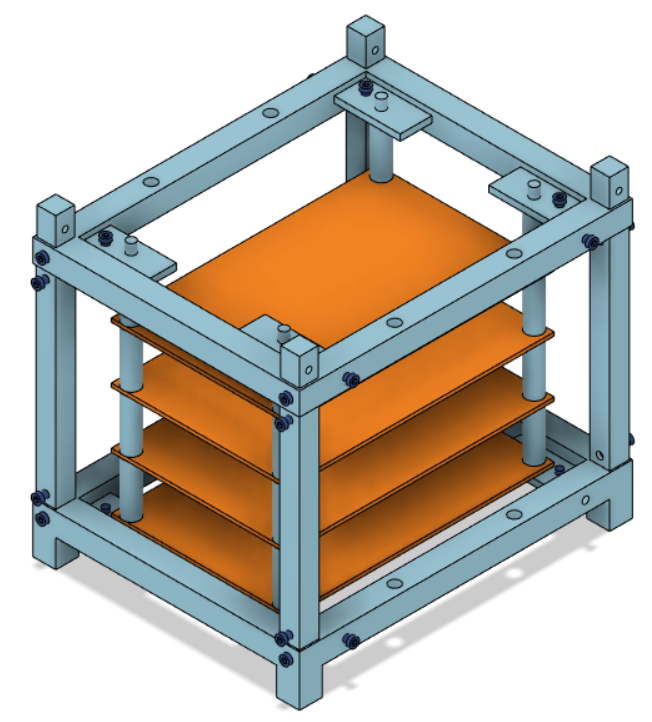
\includegraphics[width=0.48\textheight]{PlanoB.png} % Reemplaza con tu primera imagen
            \mycaption{Vista 1}
            \label{fig:Estructura1}
        \end{minipage}\hfill
        \begin{minipage}{.5\textwidth}
            \centering
            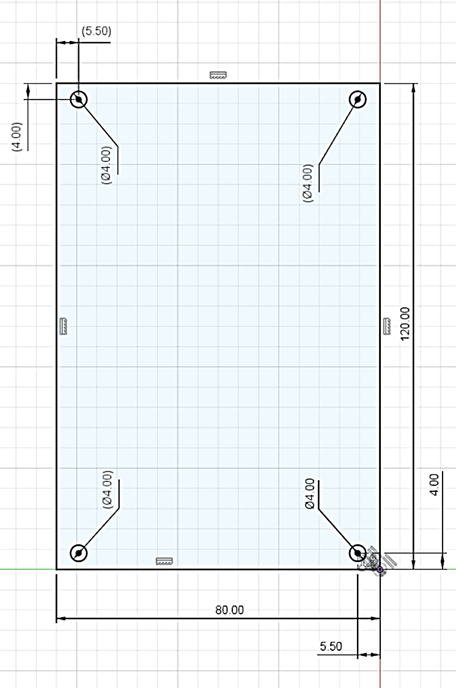
\includegraphics[width=0.45\textheight, angle=90]{PCBEspacio.png} % Reemplaza con tu segunda imagen
            \vspace*{0.25 cm}
            \mycaption{Vista 2}
            \label{fig:Estructura2}
        \end{minipage}
    \end{figure}
    \end{frame}


% PAGINA 7

\begin{frame}
    \frametitle{Resumen de Requerimientos}
    \begin{table}[!ht]
        \centering
        \caption{Requerimientos del EPS - Parte 1}
        \label{tab:requerimientos-eps-p1}
        \resizebox{\columnwidth}{!}{% Escala la tabla para que se ajuste al ancho de la columna
        \begin{tabular}{l|p{4.8cm}|p{4.8cm}|p{4.8cm}}
            \hline
            \textbf{ID} & \textbf{Descripción} & \textbf{Justificación} & \textbf{Mecanismo de verificación} \\
            \hline
            R1 & Resistencia al vacío térmico, temperatura mínima de hasta -56.50°C y 1.20\% de presión atmosférica. & Resultados en simulaciones. & Ensayos en cámara de vacío térmico \\
            \hline
            R2 & El EPS debe proveer una línea de alimentación de 3.3 V $\pm$ 1\% con una corriente mínima de 983.1 mA $\pm$ 1\%. & Bus de alimentación. & Medición de V y I.\\
            \hline
            R3 & El EPS debe proveer una línea de alimentación de 5.0 V $\pm$ 1\% con una corriente mínima de 402.30 mA $\pm$ 1\% & Bus de alimentación. & Medición de V y I. \\
            \hline
        \end{tabular}}
    \end{table}
    
    
    \end{frame}

% PAGINA 8

\begin{frame}
    \frametitle{Resumen de Requerimientos}
    \begin{table}[!ht]
        \centering
        \caption{Requerimientos del EPS - Parte 2}
        \label{tab:requerimientos-eps-p2}
        \resizebox{\columnwidth}{!}{% Escala la tabla para que se ajuste al ancho de la columna
            \begin{tabular}{l|p{4.8cm}|p{4.8cm}|p{4.8cm}}
                \hline
                \textbf{ID} & \textbf{Descripción} & \textbf{Justificación} & \textbf{Mecanismo de verificación} \\
                \hline
                R4 & No debe exceder una masa de 600 g. & Limitación de masa. & Medición de masa. \\
                \hline
                R5 & 2 PCB de 12x8 cm con 2.5 cm de altura. & Limitación de espacio. & Medición de longitud.\\
                \hline
                R6 & Registro de V [v] y I [mA]. & Función deseable. & Ensayo de registro de datos. \\
                \hline
                R7 & Registro de T [\textdegree{}C] y P [atm]. & Función deseable. & Ensayo de registro de datos. \\
                \hline
                R8 & Comunicación I2C. Recepción desde Navegación de la señal de control ON/OFF de carga útil. Transmisión de SoC a telemetría. & Integración de subsistemas. & Ensayo de comunicación. \\
                \hline
            \end{tabular}
        }
    \end{table}  
    
    \end{frame}

    % PAGINA 9

    \begin{frame}
        \frametitle{Resumen de Requerimientos}
        \begin{table}[!ht]
            \centering
            \caption{Requerimientos del EPS - Parte 3}
            \label{tab:requerimientos-eps-p3}
            \resizebox{\columnwidth}{!}{% Escala la tabla para que se ajuste al ancho de la columna
                \begin{tabular}{l|p{4.8cm}|p{4.8cm}|p{4.8cm}}
                    \hline
                    \textbf{ID} & \textbf{Descripción} & \textbf{Justificación} & \textbf{Mecanismo de verificación} \\
                    \hline
                    R9 & Control ON-OFF: carga útil.& Ahorro de energía. & Ensayo de control ON-OFF. \\
                    \hline
                    R10 & Interruptor RBF (Remove before flight, retirar antes del vuelo) para encendido y apagado del EPS.& Seguridad de la Misión, útil para prevenir accidentes. & Medición de continuidad. \\
                    \hline
                    R11 & Cargador de baterías con fuente de alimentación VDC externa & Carga del banco de baterías & Medición de voltaje. \\
                    \hline
                \end{tabular}
            }
        \end{table}
        
    \end{frame}